\documentclass[ignorenonframetext,]{beamer}
\setbeamertemplate{caption}[numbered]
\setbeamertemplate{caption label separator}{: }
\setbeamercolor{caption name}{fg=normal text.fg}
\beamertemplatenavigationsymbolsempty
\usepackage{lmodern}
\usepackage{amssymb,amsmath}
\usepackage{ifxetex,ifluatex}
\usepackage{fixltx2e} % provides \textsubscript
\ifnum 0\ifxetex 1\fi\ifluatex 1\fi=0 % if pdftex
  \usepackage[T1]{fontenc}
  \usepackage[utf8]{inputenc}
\else % if luatex or xelatex
  \ifxetex
    \usepackage{mathspec}
  \else
    \usepackage{fontspec}
  \fi
  \defaultfontfeatures{Ligatures=TeX,Scale=MatchLowercase}
\fi
\usetheme[]{CambridgeUS}
% use upquote if available, for straight quotes in verbatim environments
\IfFileExists{upquote.sty}{\usepackage{upquote}}{}
% use microtype if available
\IfFileExists{microtype.sty}{%
\usepackage{microtype}
\UseMicrotypeSet[protrusion]{basicmath} % disable protrusion for tt fonts
}{}
\newif\ifbibliography
\usepackage{longtable,booktabs}
\usepackage{caption}
% These lines are needed to make table captions work with longtable:
\makeatletter
\def\fnum@table{\tablename~\thetable}
\makeatother
\usepackage{graphicx,grffile}
\makeatletter
\def\maxwidth{\ifdim\Gin@nat@width>\linewidth\linewidth\else\Gin@nat@width\fi}
\def\maxheight{\ifdim\Gin@nat@height>\textheight0.8\textheight\else\Gin@nat@height\fi}
\makeatother
% Scale images if necessary, so that they will not overflow the page
% margins by default, and it is still possible to overwrite the defaults
% using explicit options in \includegraphics[width, height, ...]{}
\setkeys{Gin}{width=\maxwidth,height=\maxheight,keepaspectratio}

% Prevent slide breaks in the middle of a paragraph:
\widowpenalties 1 10000
\raggedbottom

\AtBeginPart{
  \let\insertpartnumber\relax
  \let\partname\relax
  \frame{\partpage}
}
\AtBeginSection{
  \ifbibliography
  \else
    \let\insertsectionnumber\relax
    \let\sectionname\relax
    \frame{\sectionpage}
  \fi
}
\AtBeginSubsection{
  \let\insertsubsectionnumber\relax
  \let\subsectionname\relax
  \frame{\subsectionpage}
}

\setlength{\parindent}{0pt}
\setlength{\parskip}{6pt plus 2pt minus 1pt}
\setlength{\emergencystretch}{3em}  % prevent overfull lines
\providecommand{\tightlist}{%
  \setlength{\itemsep}{0pt}\setlength{\parskip}{0pt}}
\setcounter{secnumdepth}{0}
\usepackage{multirow}


\newtheorem{result}{Result}

\DeclareMathOperator*{\argmin}{arg\,min}
\DeclareMathOperator*{\argmax}{arg\,max}

\newtheorem{prop}{Proposition}
\newtheorem{apptheorem}{Theorem}[section]
\newtheorem{applemma}{Lemma}[section]

\theoremstyle{definition}
\newtheorem{defn}{Definition}
\newtheorem{assumption}{Assumption}
\newtheorem{remark}{Remark}


\newcommand{\nv}{{n_{\scriptscriptstyle V}}}
\newcommand{\nh}{{n_{\scriptscriptstyle H}}}
\newcommand{\E}{E}
\newcommand{\thetaN}{\boldsymbol \theta_{\thetaidx}}
\newcommand{\thetaidx}{q(N)}

%beamer bug
\widowpenalties 1 150

\title[Model matters with RBMs]{Model matters with restricted Boltzmann machines}

\author[\href{mailto:andee.kaplan@colostate.edu}{\nolinkurl{andee.kaplan@colostate.edu}}]{Andee Kaplan}
\institute[]{Colorado State University\\
\href{mailto:andee.kaplan@colostate.edu}{\nolinkurl{andee.kaplan@colostate.edu}}}
\date[November 20, 2019]{November 20, 2019\\
~\\
Slides available at \url{http://bit.ly/kaplan-silo}\\
~\\
\footnotesize Joint work with D. Nordman and S. Vardeman}

\begin{document}
\frame{\titlepage}

\begin{frame}{What is this?}
\protect\hypertarget{what-is-this}{}

A restricted Boltzman machine (RBM) is an undirected probabilistic
graphical model with

\begin{enumerate}
\tightlist
\item
  two layers of random variables - one hidden and one visible
\item
  conditional independence within a layer (Smolensky 1986)
\end{enumerate}

\begin{figure}
\includegraphics[width=.6\linewidth]{../resources/images/rbm.png}
\caption{Hidden nodes are indicated by white circles and the visible nodes are indicated by blue circles.}
\end{figure}

\end{frame}

\begin{frame}{How is it used?}
\protect\hypertarget{how-is-it-used}{}

\begin{itemize}
\tightlist
\item
  Supervised learning, specifically image classification
\end{itemize}

\begin{figure}
\includegraphics[width=\linewidth]{../resources/images/visibles_image.pdf}
\caption{Image classification using a RBM: each image pixel comprises a node in the visible layer, $\mathcal{V}$ and the output of the RBM is used to create features passed to a supervised learning algorithm.}
\end{figure}

\end{frame}

\begin{frame}{Joint distribution}
\protect\hypertarget{joint-distribution}{}

\begin{itemize}
\item
  \(\boldsymbol x = (h_1, \dots, h_{\nh}, v_1,\dots,v_{\nv})\)
  represents visible and hidden nodes in a RBM
\item
  Each single ``binary'' random variable, visible \(v_i\) or hidden
  \(h_j\), takes values in a common coding set

  \begin{itemize}
  \tightlist
  \item
    \(\mathcal{C}=\{0,1\}\) or \(\mathcal{C}=\{-1,1\}\).
  \end{itemize}
\item
  A parametric form for probabilities

  \begin{align*} 
    \label{eqn:pmf} 
    f_{\boldsymbol \theta} (\boldsymbol x) = \frac{\exp\left(\sum\limits_{i = 1}^{\nv} \sum\limits_{j=1}^{\nh} \theta_{ij} v_i h_j + \sum\limits_{i = 1}^{\nv}\theta_{v_i} v_i + \sum\limits_{j = 1}^{\nh}\theta_{h_j} h_j\right)}{\gamma(\boldsymbol \theta)} \end{align*}

  where

  \[\gamma(\boldsymbol \theta) = \sum\limits_{\boldsymbol x \in \mathcal{C}^{\nh + \nv}}\exp\left(\sum\limits_{i = 1}^{\nv} \sum\limits_{j=1}^{\nh} \theta_{ij} v_i h_j + \sum\limits_{i = 1}^{\nv}\theta_{v_i} v_i + \sum\limits_{j = 1}^{\nh}\theta_{h_j} h_j\right)\]
\end{itemize}

\end{frame}

\begin{frame}{Deep learning}
\protect\hypertarget{deep-learning}{}

\begin{columns}[T] % align columns
\begin{column}{.48\textwidth}
\begin{itemize}
\item Stacking layers of RBMs in a deep architecture
\item Proponents claim the ability to learn "internal representations that become increasingly complex, which is considered to be a promising way of solving object and speech recognition problems" (Salakhutdinov and Hinton 2009, pp. 450).
\end{itemize}
\end{column}
\hfill
\begin{column}{.48\textwidth}
\begin{figure}
\includegraphics[width=\linewidth]{../resources/images/deep_rbm.png}
\caption{Three layer deep Boltzmann machine, with visible-to-hidden and hidden-to-hidden connections but no within-layer connections.}
\end{figure}
\end{column}
\end{columns}

\end{frame}

\begin{frame}{Why do I care?}
\protect\hypertarget{why-do-i-care}{}

\begin{enumerate}
\tightlist
\item
  The model properties are largely unexplored in the literature
\item
  The commonly cited fitting methodology remains heuristic-based
  (Hinton, Osindero, and Teh 2006)
\end{enumerate}

We want to

\begin{enumerate}
\tightlist
\item
  Provide steps toward understanding properties of the model class from
  the perspective of statistical theory
\item
  Explore the possibility of a rigorous fitting methodology
\end{enumerate}

\end{frame}

\begin{frame}{}
\protect\hypertarget{section}{}

\begin{center}
\Huge{Properties of RBM Model Class}
\end{center}

\end{frame}

\begin{frame}{Degeneracy, instability, and uninterpretability. Oh my!}
\protect\hypertarget{degeneracy-instability-and-uninterpretability.-oh-my}{}

The highly flexible nature of a RBM (\(\nh + \nv + \nh*\nv\) parameters)
makes at least three kinds of potential model impropriety of concern

\begin{enumerate}
\tightlist
\item
  \emph{degeneracy}
\item
  \emph{instability}, and
\item
  \emph{uninterpretability}
\end{enumerate}

\begin{quote}
A model should ``provide an explanation of the mechanism underlying the
observed phenomena'' (G. E. P. Box 1967).
\end{quote}

RBMs often

\begin{itemize}
\tightlist
\item
  fail to generate data with realistic variability and thus an
  unsatisfactory conceptualization of the data generation process (Li
  2014)
\item
  exhibit model instability (over-sensitivity) (Szegedy et al. 2013;
  Nguyen, Yosinski, and Clune 2014)
\end{itemize}

\end{frame}

\begin{frame}{Near-degeneracy}
\protect\hypertarget{near-degeneracy}{}

\begin{definition}[Model Degeneracy]
A disproportionate amount of probability is placed on only a few elements of the sample space, $\mathcal{C}^{\nh + \nv}$, by the model.
\end{definition}

RBM models exhibit \emph{near-degeneracy} when random variables in
\[Q_{\boldsymbol \theta}(\boldsymbol x) = \sum\limits_{i = 1}^{\nv} \sum\limits_{j=1}^{\nh} \theta_{ij} v_i h_j + \sum\limits_{i = 1}^\nv\theta_{v_i} v_i + \sum\limits_{j = 1}^\nh\theta_{h_j} h_j,
\] have a mean vector \(\boldsymbol \mu(\boldsymbol \theta)\) close to
the boundary of the convex hull of
\(\mathcal{T} = \{\boldsymbol t(x): x \in \mathcal{C}^{\nh + \nv}\}\)
(Handcock 2003), where
\[\boldsymbol t(\boldsymbol x) = \{v_1, \dots, v_{\nv}, h_1, \dots, h_{\nh}, v_1 h_1, \dots, v_{\nv} h_{\nh} \}\]
and
\[\boldsymbol \mu(\boldsymbol \theta) = \text{E}_{\boldsymbol \theta} \boldsymbol t(\boldsymbol X)\].

\end{frame}

\begin{frame}{Instability}
\protect\hypertarget{instability}{}

\begin{definition}[Instability]
Characterized by excessive sensitivity in the model, where small changes in the components of data outcomes, $\boldsymbol x$, lead to substantial changes in probability.
\end{definition}

\begin{itemize}
\tightlist
\item
  Concept of model deficiency related to \emph{instability} for a class
  of exponential families of distributions (Schweinberger 2011)
\item
  For the RBM, consider how model incorporates more visibles

  \begin{itemize}
  \tightlist
  \item
    Model parameters in a longer sequence
    \(\boldsymbol \theta_{\nv} \in \mathbb{R}^{\nv + \nh + \nv*\nh}, \nv \ge 1\)
  \item
    May also arbitrarily expand the number of hidden variables used
  \end{itemize}
\end{itemize}

\end{frame}

\begin{frame}{Unstable RBMs}
\protect\hypertarget{unstable-rbms}{}

\begin{definition}[S-unstable RBM]
A RBM model formulation is \emph{S-unstable} if
\begin{align*}
\lim\limits_{\nv \rightarrow \infty} \frac{1}{\nv} \text{LREP}(\boldsymbol \theta_{\nv}) = \infty.
\end{align*}
where 
\begin{align}
\label{eqn:elpr}
\text{LREP}(\boldsymbol \theta_{\nv}) = \log \left[\frac{\max\limits_{(v_1, \dots, v_{\nv}) \in \mathcal{C}^\nv}P_{\boldsymbol \theta_\nv}(v_1, \dots, v_\nv)}{\min\limits_{(v_1, \dots, v_\nv) \in \mathcal{C}^\nv}P_{\boldsymbol \theta_\nv}(v_1, \dots, v_\nv)}\right]
\end{align}
\end{definition}

S-unstable RBM models are undesirable for several reasons - small
changes in data outcomes can lead to overly-sensitive changes in
probability.

\end{frame}

\begin{frame}{One-pixel change}
\protect\hypertarget{one-pixel-change}{}

Consider the biggest log-probability ratio for a one-pixel (one
component) change in visibles (data outcomes)

\[
\Delta(\boldsymbol \theta_\nv) \equiv \max \left\{\log \frac{P_{\boldsymbol \theta_\nv}(v_1, \dots, v_\nv)}{P_{\boldsymbol \theta_\nv}(v_1^*, \dots, v_\nv^*)} \right\},
\]

where
\((v_1, \dots, v_\nv) \& (v_1^*, \dots, v_\nv^*) \in \mathcal{C}^\nv\)
differ by exactly one component

\begin{result}
\label{prop:instab}
Let $c > 0$ and fix an integer $\nv \ge 1$. If $\frac{1}{\nv}\text{LREP}(\boldsymbol \theta_\nv) > c$, then $\Delta(\boldsymbol \theta_\nv) > c$.
\end{result}

If the \(\nv^{-1}LREP(\boldsymbol\theta_{\nv})\) is too large, then a
RBM model will exhibit large probability shifts for very small changes
in the data configuration.

\end{frame}

\begin{frame}{Tie to degeneracy}
\protect\hypertarget{tie-to-degeneracy}{}

Define an arbitrary modal set of possible outcomes (i.e.~set of highest
probability outcomes) for a given \(0 < \epsilon < 1\) as

\small

\begin{align*}
M_{\epsilon, \boldsymbol \theta_\nv} \equiv \left\{\boldsymbol v \in \mathcal{C}^\nv: \log P_{\boldsymbol \theta_\nv}(\boldsymbol v) > (1-\epsilon)\max\limits_{\boldsymbol v^*}P_{\boldsymbol \theta_\nv}(\boldsymbol v^*) + \epsilon\min\limits_{\boldsymbol v^*}P_{\boldsymbol \theta_\nv}(\boldsymbol v^*) \right\}
\end{align*} \normalsize

\begin{result}
\label{prop:degen}
For an S-unstable RBM model, and for any given $0 < \epsilon < 1$, $P_{\boldsymbol \theta_\nv}\left((v_1, \dots, v_\nv) \in M_{\epsilon, \boldsymbol \theta_\nv}\right) \rightarrow 1$ holds as $\nv \rightarrow \infty$.
\end{result}

\begin{itemize}
\tightlist
\item
  All probability will stack up on mode sets or potentially those few
  outcomes with the highest probability
\end{itemize}

\end{frame}

\begin{frame}{Uninterpretability}
\protect\hypertarget{uninterpretability}{}

\begin{definition}[Uninterpretability]
Characterized by marginal mean-structure (controlled by main effect parameters $\theta_{v_i}, \theta_{h_j}$) not being maintained in the model due to dependence (interaction parameters $\theta_{ij}$) (Kaiser 2007).
\end{definition}

\begin{itemize}
\tightlist
\item
  Model expectations,
  E\(\left[\boldsymbol X | \boldsymbol \theta\right]\)
\item
  Expectations given independence,
  E\(\left[\boldsymbol X | \boldsymbol \theta^* \right]\), where
  \(\boldsymbol \theta^*\) matches \(\boldsymbol \theta\) for all main
  effects but otherwise has \(\theta_{ij} = 0\) for
  \(i = 1, \dots, \nv, j = 1, \dots, \nh\)
\item
  If
  \(|\text{E}\left[\boldsymbol X | \boldsymbol \theta\right] - \text{E}\left[\boldsymbol X | \boldsymbol \theta^*\right]|\)
  is large then the RBM with parameter vector \(\boldsymbol \theta\) is
  \emph{uninterpetable}
\end{itemize}

\end{frame}

\begin{frame}{FOES models}
\protect\hypertarget{foes-models}{}

Statements about near-degeneracy, instability, and uninterpretability
hold for a general class of models that includes the RBM.

\begin{itemize}
\item
  \(\boldsymbol X_N = (X_1, \dots, X_N)\) collection of discrete random
  variables with a finite sample space
\item
  \(\mathcal{X}^N\) finite sample space, represented as some \(N\)-fold
  Cartesian product
\item
  \(P_{{\thetaN}}\) probability model on \(\mathcal{X}^N\) for each
  \(N\)
\item
  Assume that the model support of \(P_{{\thetaN}}\) is the sample space
  \(\mathcal{X}^N\).
\end{itemize}

\begin{block}{Definition}

This framework produces \emph{Finite Outcome Everywhere Supported
(FOES)} models, \(P_{{\thetaN}}\), indexed by a defining sequence of
parameters \({\thetaN}\), to describe data \(\boldsymbol X_N\) of any
given sample size \(N \geq 1\).

(Kaplan, Nordman, and Vardeman 2019a)

\end{block}

\end{frame}

\begin{frame}{Examples}
\protect\hypertarget{examples}{}

\begin{itemize}
\item
  Discrete exponential family models
\item
  Discrete restricted Boltzmann machines
\item
  Binary deep learning models

  \vspace{.1in}

  \begin{enumerate}
  \tightlist
  \item
    \textbf{Deep Boltzmann machine (DBM).} Conditional independence
    within all layers, stacked RBM models with conditional dependence
    between neighboring layers
  \end{enumerate}

  \vspace{.1in}

  \begin{enumerate}
  \setcounter{enumi}{1}
  \tightlist
  \item
    \textbf{Deep belief network (DBN).} Multiple layers of latent random
    variables stacked in a deep architecture with no conditional
    dependence between layers; all but the last stacked layer are
    Bayesian networks (directed dependence), rather than RBMs
  \end{enumerate}
\end{itemize}

\end{frame}

\begin{frame}{Avoiding S-instability for the RBM}
\protect\hypertarget{avoiding-s-instability-for-the-rbm}{}

Based on the definition of S-instability, we can show how an S-unstable
distribution can arise (and potentially how to avoid this).

\begin{itemize}
\tightlist
\item
  All instability in the marginal RBM model for the data
  \(\boldsymbol X\) can be attributed to large magnitudes (or many
  terms) of \(\boldsymbol \theta_{v}\) and/or
  \(\boldsymbol \theta_{interaction}\)
\item
  An S-unstable marginal model implies an S-unstable joint model
\item
  Further potential causes of S-instability exist for the joint model,
  often due to the size of \(|\boldsymbol \theta_{v}|_1\)
\end{itemize}

\begin{block}{Key Finding}

To prevent instability in the joint model of an RBM (and all models that
embloy RBMs, e.g.~a DBM), the combined magnitudes of all parameters
\(\boldsymbol \theta\) must be controlled.

\end{block}

\end{frame}

\begin{frame}{Visualizing properties in manageable (a.k.a. small) RBMs}
\protect\hypertarget{visualizing-properties-in-manageable-a.k.a.-small-rbms}{}

\begin{itemize}
\tightlist
\item
  To explore the effects of RBM parameters \(\boldsymbol \theta\) on
  \emph{near-degeneracy}, \emph{instability}, and
  \emph{uninterpretability}, consider models of small size\\
\item
  For \(\nh, \nv \in \{1, \dots, 4\}\), sample 100 values of
  \(\boldsymbol \theta\)

  \begin{enumerate}
  \tightlist
  \item
    Split \(\boldsymbol \theta\) into
    \(\boldsymbol \theta_{interaction}\) and
    \(\boldsymbol \theta_{main}\)
  \item
    Allow the two types of terms to have varying average magnitudes,
    \(||\boldsymbol \theta_{main} || /(\nh+\nv)\) and
    \(||\boldsymbol \theta_{interaction} || /(\nh*\nv)\)
  \item
    Average magnitudes vary on a grid between 0.001 and 3 with 24
    breaks, yielding 576 grid points
  \end{enumerate}
\item
  Calculate metrics of model impropriety,
  \(\boldsymbol \mu(\boldsymbol \theta)\),
  \(\text{LREP}(\boldsymbol \theta)/\nv\), and the coordinates of
  \(\left|\text{E}\left[\boldsymbol X | \boldsymbol \theta\right] - \text{E}\left[\boldsymbol X | \boldsymbol \theta^* \right] \right|\).
\item
  In the case of \emph{near-degeneracy}, classify each model as
  near-degenerate or ``viable'' based on the distance of
  \(\boldsymbol \mu(\boldsymbol \theta)\) from the boundary of the
  convex hull of \(\mathcal{T}\)
\end{itemize}

\end{frame}

\begin{frame}{Simulation results}
\protect\hypertarget{simulation-results}{}

\begin{figure}
\includegraphics[width=.32\linewidth]{slides_files/figure-beamer/unnamed-chunk-1-1} \includegraphics[width=.32\linewidth]{slides_files/figure-beamer/unnamed-chunk-1-2} \includegraphics[width=.32\linewidth]{slides_files/figure-beamer/unnamed-chunk-1-3} \caption{\label{fig:degen_plots}The fraction of models that were near-degenerate (left), the sample mean value of $\text{LREP}(\boldsymbol \theta)/\nv$ (middle), and the sample mean of the maximum component of the absolute difference between the model expectation vector, E$\left[\boldsymbol X | \boldsymbol \theta\right]$, and the expectation vector given independence, E$\left[\boldsymbol X | \boldsymbol \theta^* \right ]$ (right).}\label{fig:unnamed-chunk-1}
\end{figure}

\end{frame}

\begin{frame}{}
\protect\hypertarget{section-1}{}

\begin{center}
\Huge{Rigorous Fitting Methodology}
\end{center}

\end{frame}

\begin{frame}{Model fitting}
\protect\hypertarget{model-fitting}{}

\begin{enumerate}
\tightlist
\item
  Computational concerns: Fitting a RBM via maximum likelihood (ML)
  methods infeasible due to the intractibility of the normalizing term
  \(\gamma(\boldsymbol \theta)\)

  \begin{itemize}
  \tightlist
  \item
    Ad hoc methods used to avoid this problem with stochastic ML
  \item
    Employ a small number of MCMC draws to approximate
    \(\gamma(\boldsymbol \theta)\)
  \end{itemize}
\item
  Model parameterization concerns: With enough hiddens,

  \begin{itemize}
  \tightlist
  \item
    Potential to re-create any distribution for the data (Le Roux and
    Bengio 2008; Montufar and Ay 2011; and Montúfar, Rauh, and Ay 2011)

    \begin{itemize}
    \tightlist
    \item
      The model for the cell probabilities that has the highest
      likelihood over \emph{all possible model classes} is the empirical
      distribution
    \item
      The RBM model ensures that this empirical distribution can be
      arbitrarily well approximated
    \end{itemize}
  \item
    When empirical distribution contains empty cells, ML will chase
    parameters to \(\infty\) in order to zero out corresponding RBM cell
    probabilities
  \end{itemize}
\end{enumerate}

\end{frame}

\begin{frame}{Bayesian methods}
\protect\hypertarget{bayesian-methods}{}

\begin{itemize}
\tightlist
\item
  Consider what might be done in a principled manner, small test
\item
  To avoid model impropriety, avoid parts of the parameter space
  \(\mathbb{R}^{\nv + \nh + \nv*\nh}\) leading to
  \emph{near-degeneracy}, \emph{instability}, and
  \emph{uninterpretability}.

  \begin{itemize}
  \tightlist
  \item
    Shrink \(\boldsymbol \theta\) toward \(\boldsymbol 0\)

    \begin{enumerate}
    \tightlist
    \item
      Specify priors that place low probability on large values of
      \(||\boldsymbol \theta||\)
    \item
      Shrink \(\boldsymbol \theta_{interaction}\) more than
      \(\boldsymbol \theta_{main}\)
    \end{enumerate}
  \end{itemize}
\item
  Consider a test case with \(\nv = \nh = 4\)

  \begin{itemize}
  \tightlist
  \item
    \(\boldsymbol \theta\) chosen as a sampled value from a grid point
    in figure \ref{fig:degen_plots} with \(< 5\)\% near-degeneracy (not
    near the convex hull of the sufficient statistics)
  \item
    simulate \(n = 5,000\) as a training set and fit the RBM using three
    Bayes methodologies
  \end{itemize}
\end{itemize}

\end{frame}

\begin{frame}{Fitting methodologies}
\protect\hypertarget{fitting-methodologies}{}

\begin{enumerate}
\tightlist
\item
  \emph{A ``trick'' prior (BwTPLV)}

  \begin{itemize}
  \tightlist
  \item
    Cancel out normalizing term in the likelihood
  \item
    Resulting full conditionals of \(\boldsymbol \theta\) are
    multivariate Normal
  \item
    \(h_j\) are carried along as latent variables \begin{align*}
     \pi(\boldsymbol \theta) \propto \gamma(\boldsymbol \theta)^n \exp\left(-\frac{1}{2C_{1}}\boldsymbol \theta_{main}'\boldsymbol \theta_{main} -\frac{1}{2C_{2}}\boldsymbol \theta_{interaction}'\boldsymbol \theta_{interaction}\right), \vspace{-.75cm}
     \end{align*} where \(C_{2} < C_{1}\) (Li 2014)
  \end{itemize}
\end{enumerate}

\end{frame}

\begin{frame}{Fitting methodologies (cont'd)}
\protect\hypertarget{fitting-methodologies-contd}{}

\begin{enumerate}
\setcounter{enumi}{1}
\tightlist
\item
  \emph{A truncated Normal prior (BwTNLV)}

  \begin{itemize}
  \tightlist
  \item
    Independent spherical normal distributions as priors for
    \(\boldsymbol \theta_{main}\) and
    \(\boldsymbol \theta_{interaction}\)

    \begin{itemize}
    \tightlist
    \item
      \(\sigma_{interaction} < \sigma_{main}\)
    \item
      \emph{truncated} at \(3\sigma_{main}\) and
      \(3\sigma_{interaction}\), respectively
    \end{itemize}
  \item
    Simulation from the posterior using a geometric adaptive MH step
    (Zhou 2014)
  \item
    \(h_j\) are carried along in the MCMC implementation as latent
    variables
  \end{itemize}
\item
  \emph{A truncated Normal prior and marginalized likelihood (BwTNML)}

  \begin{itemize}
  \tightlist
  \item
    Marginalize out \(\boldsymbol h\) in
    \(f_{\boldsymbol \theta}(\boldsymbol x)\)
  \item
    Use the truncated Normal priors applied to the marginal
    probabilities for visible variables (recall visibles are the
    observed data, hiddens are not)
  \end{itemize}
\end{enumerate}

\end{frame}

\begin{frame}{Hyperparameters}
\protect\hypertarget{hyperparameters}{}

\begin{table}[ht]
\centering
\caption{The values used for the hyperparameters for all three fitting methods. A rule of thumb is imposed which decreases prior variances for the model parameters as the size of the model increases and also shrinks $\boldsymbol \theta_{interaction}$ more than $\boldsymbol \theta_{main}$. The common $C$ defining $C_1$ and $C_2$  in the BwTPLV method is chosen by tuning.}
\label{tab:hyperparam}
\begin{tabular}{|l|c|c|}
\hline 
Method & Hyperparameter & Value \\ 
\hline \hline
\multirow{2}{*}{BwTPLV} & $C_1$ & $\frac{C}{n}\frac{1}{\nh + \nv}$ \\
 & $C_2$ & $\frac{C}{n}\frac{1}{\nh*\nv}$ \\
\hline
\multirow{2}{*}{BwTNLV} & $\sigma^2_{main}$ & $\frac{1}{\nh + \nv}$ \\
 & $\sigma^2_{interaction}$ & $\frac{1}{\nh*\nv}$ \\
\hline
\multirow{2}{*}{BwTNML} & $\sigma^2_{main}$ & $\frac{1}{\nh + \nv}$ \\
 & $\sigma^2_{interaction}$ & $\frac{1}{\nh*\nv}$ \\
\hline
\end{tabular}
\end{table}

\end{frame}

\begin{frame}{Mixing}
\protect\hypertarget{mixing}{}

The BwTNLV (2) and the BwTNML method (3) are drawing from the same
stationary posterior distribution for images.

\begin{figure}
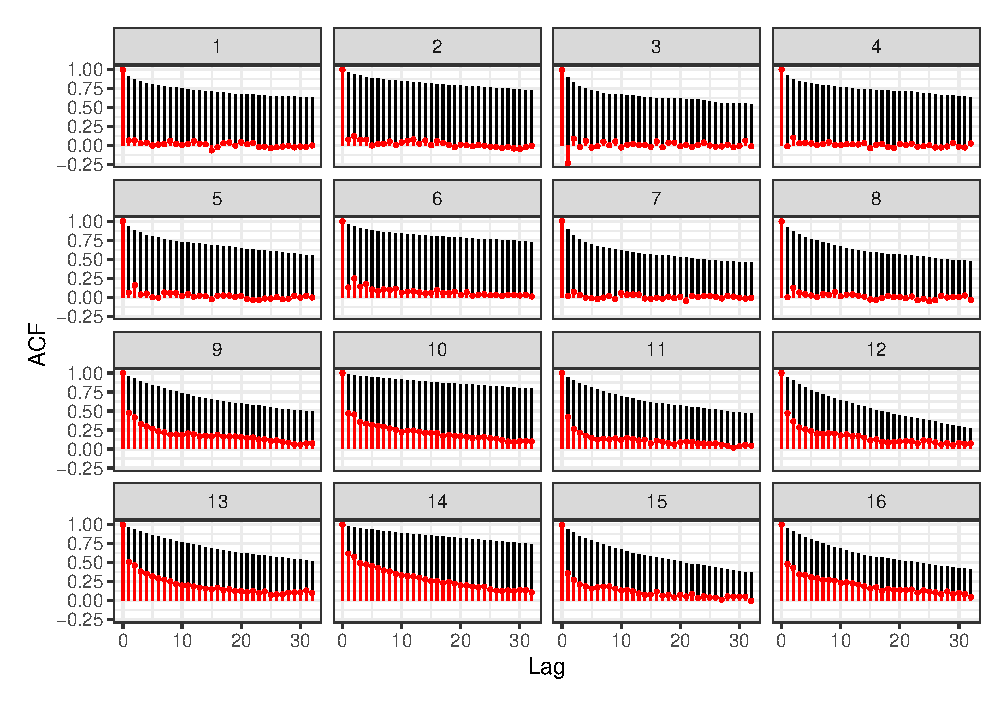
\includegraphics[width=.7\linewidth]{slides_files/figure-beamer/acf-1} \caption{\label{fig:acf}The autocorrelation functions (ACF) for the posterior probabilities of all $2^4 = 16$ possible outcomes for the vector of $4$ visibles assessed at multiple lags for each method with BwTNLV in black and BwTNML in red.}\label{fig:acf}
\end{figure}

\end{frame}

\begin{frame}{Effective sample size}
\protect\hypertarget{effective-sample-size}{}

\begin{itemize}
\tightlist
\item
  Overlapping blockmeans approach (Gelman, Shirley, and others 2011)

  \begin{itemize}
  \tightlist
  \item
    Crude estimate for the aysmptotic variance of the probability of
    each image
  \item
    Compare it to an estimate of the asymptotic variance assuming IID
    draws from the target distribution
  \end{itemize}
\end{itemize}

\tiny

\begin{longtable}[]{@{}rrrrrr@{}}
\caption{\label{tab:m_eff}The effective sample sizes for a chain of
length \(M = 1000\) regarding all \(16\) probabilities for possible
vector outcomes of visibles. BwTNLV would require at least \(4.7\) times
as many MCMC iterations to achieve the same amount of effective
information about the posterior distribution.}\tabularnewline
\toprule
Outcome & BwTNLV & BwTNML & Outcome & BwTNLV & BwTNML\tabularnewline
\midrule
\endfirsthead
\toprule
Outcome & BwTNLV & BwTNML & Outcome & BwTNLV & BwTNML\tabularnewline
\midrule
\endhead
1 & 73.00 & 509.43 & 9 & 83.47 & 394.90\tabularnewline
2 & 65.05 & 472.51 & 10 & 95.39 & 327.35\tabularnewline
3 & 87.10 & 1229.39 & 11 & 70.74 & 356.56\tabularnewline
4 & 72.64 & 577.73 & 12 & 81.40 & 338.30\tabularnewline
5 & 71.67 & 452.01 & 13 & 105.98 & 373.59\tabularnewline
6 & 66.49 & 389.78 & 14 & 132.61 & 306.91\tabularnewline
7 & 84.30 & 660.37 & 15 & 82.15 & 365.30\tabularnewline
8 & 75.46 & 515.09 & 16 & 98.05 & 304.57\tabularnewline
\bottomrule
\end{longtable}

\end{frame}

\begin{frame}{Posterior distributions of images}
\protect\hypertarget{posterior-distributions-of-images}{}

\begin{figure}
\centering
\includegraphics{slides_files/figure-beamer/fitting_plot-1.pdf}
\caption{\label{fig:fitting_plot}Posterior probabilities of \(16 = 2^4\)
possible realizations of \(4\) visibles using two of the three Bayesian
fitting techniques, BwTPLV and BwTNML. Black lines show true
probabilities of each vector of visibles based on the parameters used to
generate the training data while red lines show the empirical
distribution.}
\end{figure}

\end{frame}

\begin{frame}{Wrapping up}
\protect\hypertarget{wrapping-up}{}

\begin{itemize}
\tightlist
\item
  RBMs shown success for classification, but concerning as statistical
  models due to \emph{near-degeneracy}, \emph{S-instability}, and
  \emph{uninterpretability}
\item
  Rigorous fitting methodology is difficult

  \begin{itemize}
  \tightlist
  \item
    Numerical complications in likelihood maximization may occur due to
    degeneracy and S-instability when all probability in pushed to
    opposite extremes in the sample space
  \item
    For Bayesian inference, S-instability may hinder effective chain
    mixing
  \end{itemize}
\item
  RBMs questionably useful as any distribution for the visibles can be
  approximated arbitrarily well

  \begin{itemize}
  \tightlist
  \item
    The empirical distribution of visibles is the best fitting model for
    observed cell data
  \item
    There can be no ``smoothed distribution'' achieved in a RBM model of
    sufficient size with a rigorous likelihood-based method
  \end{itemize}
\end{itemize}

Skeptical that any model built using RBMs (e.g., DBM) can achieve useful
\textbf{inference} in principled way without limiting flexibility of the
fitted model

\end{frame}

\begin{frame}{Relevant papers}
\protect\hypertarget{relevant-papers}{}

\vfill

\begin{enumerate}
\tightlist
\item
  Kaplan, Andee, Daniel Nordman, and Stephen Vardeman. ``Properties and
  Bayesian fitting of restricted Boltzmann machines.'' \emph{Statistical
  Analysis and Data Mining: The ASA Data Science Journal} 12.1 (2019):
  23-38.
\end{enumerate}

\vspace{0.25in}

\begin{enumerate}
\setcounter{enumi}{1}
\tightlist
\item
  Kaplan, Andee, Daniel J. Nordman, and Stephen B. Vardeman. ``On the
  S-instability and degeneracy of discrete deep learning models.''
  \emph{Information and Inference: A Journal of the IMA} (2019).
\end{enumerate}

\vfill

\end{frame}

\begin{frame}{Thank you}
\protect\hypertarget{thank-you}{}

\begin{itemize}
\item
  Slides -- \url{http://bit.ly/kaplan-silo}
\item
  Contact

  \begin{itemize}
  \tightlist
  \item
    Email --
    \href{mailto:andee.kaplan@colostate.edu}{\nolinkurl{andee.kaplan@colostate.edu}}
  \item
    Twitter -- \url{http://twitter.com/andeekaplan}
  \item
    GitHub -- \url{http://github.com/andeek}
  \end{itemize}
\end{itemize}

\end{frame}

\begin{frame}{Appendix: Parameters used}
\protect\hypertarget{appendix-parameters-used}{}

\scriptsize

\begin{longtable}[]{@{}lrlrlr@{}}
\caption{\label{tab:theta}Parameters used to fit a test case with
\(\nv = \nh = 4\). This parameter vector was chosen as a sampled value
of \(\boldsymbol \theta\) that was not near the convex hull of the
sufficient statistics for a grid point in figure \ref{fig:degen_plots}
with \(< 5\)\% near-degeneracy.}\tabularnewline
\toprule
Parameter & Value & Parameter & Value & Parameter & Value\tabularnewline
\midrule
\endfirsthead
\toprule
Parameter & Value & Parameter & Value & Parameter & Value\tabularnewline
\midrule
\endhead
\(\theta_{v1}\) & -1.1043760 & \(\theta_{11}\) & -0.0006334 &
\(\theta_{31}\) & -0.0038301\tabularnewline
\(\theta_{v2}\) & -0.2630044 & \(\theta_{12}\) & -0.0021401 &
\(\theta_{32}\) & 0.0032237\tabularnewline
\(\theta_{v3}\) & 0.3411915 & \(\theta_{13}\) & 0.0047799 &
\(\theta_{33}\) & 0.0020681\tabularnewline
\(\theta_{v4}\) & -0.2583769 & \(\theta_{14}\) & 0.0025282 &
\(\theta_{34}\) & 0.0041429\tabularnewline
\(\theta_{h1}\) & -0.1939302 & \(\theta_{21}\) & 0.0012975 &
\(\theta_{41}\) & 0.0089533\tabularnewline
\(\theta_{h2}\) & -0.0572858 & \(\theta_{22}\) & 0.0000253 &
\(\theta_{42}\) & -0.0042403\tabularnewline
\(\theta_{h3}\) & -0.2101802 & \(\theta_{23}\) & -0.0004352 &
\(\theta_{43}\) & -0.0000480\tabularnewline
\(\theta_{h4}\) & 0.2402456 & \(\theta_{24}\) & -0.0086621 &
\(\theta_{44}\) & 0.0004767\tabularnewline
\bottomrule
\end{longtable}

\end{frame}

\begin{frame}[allowframebreaks]{References}
\protect\hypertarget{references}{}

\tiny

\hypertarget{refs}{}
\leavevmode\hypertarget{ref-gelman2011inference}{}%
Gelman, Andrew, Kenneth Shirley, and others. 2011. ``Inference from
Simulations and Monitoring Convergence.'' \emph{Handbook of Markov Chain
Monte Carlo}, 163--74.

\leavevmode\hypertarget{ref-box1967discrimination}{}%
G. E. P. Box, W. J. Hill. 1967. ``Discrimination Among Mechanistic
Models.'' \emph{Technometrics} 9 (1). {[}Taylor \& Francis, Ltd.,
American Statistical Association, American Society for Quality{]}:
57--71.

\leavevmode\hypertarget{ref-handcock2003assessing}{}%
Handcock, Mark S. 2003. ``Assessing Degeneracy in Statistical Models of
Social Networks.'' Center for Statistics; the Social Sciences,
University of Washington. \url{http://www.csss.washington.edu/}.

\leavevmode\hypertarget{ref-hinton2006fast}{}%
Hinton, Geoffrey E, Simon Osindero, and Yee-Whye Teh. 2006. ``A Fast
Learning Algorithm for Deep Belief Nets.'' \emph{Neural Computation} 18
(7). MIT Press: 1527--54.

\leavevmode\hypertarget{ref-kaiser2007statistical}{}%
Kaiser, Mark S. 2007. ``Statistical Dependence in Markov Random Field
Models.'' \emph{Statistics Preprints} Paper 57. Digital Repository @
Iowa State University.
\url{http://lib.dr.iastate.edu/stat_las_preprints/57/}.

\leavevmode\hypertarget{ref-kaplan2016note}{}%
Kaplan, Andee, Daniel J Nordman, and Stephen B Vardeman. 2019a. ``On the
S-instability and degeneracy of discrete deep learning models.''
\emph{Information and Inference: A Journal of the IMA}, November.
\url{https://doi.org/10.1093/imaiai/iaz022}.

\leavevmode\hypertarget{ref-kaplan2019properties}{}%
Kaplan, Andee, Daniel Nordman, and Stephen Vardeman. 2019b. ``Properties
and Bayesian Fitting of Restricted Boltzmann Machines.''
\emph{Statistical Analysis and Data Mining: The ASA Data Science
Journal} 12 (1): 23--38. \url{https://doi.org/10.1002/sam.11396}.

\leavevmode\hypertarget{ref-le2008representational}{}%
Le Roux, Nicolas, and Yoshua Bengio. 2008. ``Representational Power of
Restricted Boltzmann Machines and Deep Belief Networks.'' \emph{Neural
Computation} 20 (6). MIT Press: 1631--49.

\leavevmode\hypertarget{ref-li2014biclustering}{}%
Li, Jing. 2014. ``Biclustering Methods and a Bayesian Approach to
Fitting Boltzmann Machines in Statistical Learning.'' PhD thesis, Iowa
State University; Graduate Theses; Dissertations.
\url{http://lib.dr.iastate.edu/etd/14173/}.

\leavevmode\hypertarget{ref-montufar2011refinements}{}%
Montufar, Guido, and Nihat Ay. 2011. ``Refinements of Universal
Approximation Results for Deep Belief Networks and Restricted Boltzmann
Machines.'' \emph{Neural Computation} 23 (5). MIT Press: 1306--19.

\leavevmode\hypertarget{ref-montufar2011expressive}{}%
Montúfar, Guido F, Johannes Rauh, and Nihat Ay. 2011. ``Expressive Power
and Approximation Errors of Restricted Boltzmann Machines.'' In
\emph{Advances in Neural Information Processing Systems}, 415--23. NIPS.

\leavevmode\hypertarget{ref-nguyen2014deep}{}%
Nguyen, Anh Mai, Jason Yosinski, and Jeff Clune. 2014. ``Deep Neural
Networks Are Easily Fooled: High Confidence Predictions for
Unrecognizable Images.'' \emph{arXiv Preprint arXiv:1412.1897}.
\url{http://arxiv.org/abs/1412.1897}.

\leavevmode\hypertarget{ref-salakhutdinov2009deep}{}%
Salakhutdinov, Ruslan, and Geoffrey E Hinton. 2009. ``Deep Boltzmann
Machines.'' In \emph{International Conference on Artificial Intelligence
and Statistics}, 448--55. AI \& Statistics.

\leavevmode\hypertarget{ref-schweinberger2011instability}{}%
Schweinberger, Michael. 2011. ``Instability, Sensitivity, and Degeneracy
of Discrete Exponential Families.'' \emph{Journal of the American
Statistical Association} 106 (496). Taylor \& Francis: 1361--70.

\leavevmode\hypertarget{ref-smolensky1986information}{}%
Smolensky, Paul. 1986. ``Information Processing in Dynamical Systems:
Foundations of Harmony Theory.'' DTIC Document.

\leavevmode\hypertarget{ref-szegedy2013intriguing}{}%
Szegedy, Christian, Wojciech Zaremba, Ilya Sutskever, Joan Bruna,
Dumitru Erhan, Ian J. Goodfellow, and Rob Fergus. 2013. ``Intriguing
Properties of Neural Networks.'' \emph{arXiv Preprint arXiv:1312.6199}.
\url{http://arxiv.org/abs/1312.6199}.

\leavevmode\hypertarget{ref-zhou2014some}{}%
Zhou, Wen. 2014. ``Some Bayesian and Multivariate Analysis Methods in
Statistical Machine Learning and Applications.'' PhD thesis, Iowa State
University; Graduate Theses; Dissertations.
\url{http://lib.dr.iastate.edu/etd/13816/}.

\end{frame}

\end{document}
